\documentclass[a4paper]{article}

\usepackage{amsmath}
\usepackage{amssymb}
\usepackage[english]{babel}
\usepackage[a4paper,includeheadfoot,margin=2.54cm]{geometry}
\usepackage{graphicx}
\usepackage{hyperref}
\usepackage[utf8]{inputenc}
\usepackage{listings}
\usepackage{todonotes}
\usepackage{url}
\usepackage{xspace}


% XXX: Maybe avoid xspace
\newcommand{\tray}{$\mathit{Tray}$\xspace}
\newcommand{\recipeOne}{$\mathit{Recipe}_1$\xspace}
\newcommand{\recipeTwo}{$\mathit{Recipe}_2$\xspace}
\newcommand{\recipeThree}{$\mathit{Recipe}_3$\xspace}
\newcommand{\robotOne}{$\mathit{Robot}_1$\xspace}
\newcommand{\robotTwo}{$\mathit{Robot}_2$\xspace}
\newcommand{\robotThree}{$\mathit{Robot}_3$\xspace}
\newcommand{\robotSwap}{$\mathit{Swap}$\xspace}
\newcommand{\chuckIn}{$\mathit{In}$\xspace}
\newcommand{\chuckOut}{$\mathit{Out}$\xspace}
\newcommand{\chuckEmptyOne}{$\mathit{Empty}_1$\xspace}
\newcommand{\chuckEmptyTwo}{$\mathit{Empty}_2$\xspace}
\newcommand{\chuckA}{$A$\xspace}
\newcommand{\chuckB}{$B$\xspace}
\newcommand{\chuckMeas}{$\mathit{Meas}$\xspace}
\newcommand{\chuckProj}{$\mathit{Proj}$\xspace}


\lstdefinelanguage{mcrl2}{
    morecomment=[l]{\%},
    morekeywords=[1]{sort, cons, map, var, eqn, act, proc, init, struct},
    morekeywords=[2]{delta, tau, true, false},
    morekeywords=[3]{sum, block, allow, hide, rename, comm},
    morekeywords=[4]{whr, end, lambda, forall, exists, div, mod, in, val},
    morekeywords=[5]{Bool, Pos, Nat, Int, Real, List, Set, Bag},
    morekeywords=[6]{Position,Recipe,Robot,ChuckStatus,RobotPositionT},
    sensitive=true,
}[keywords, comments]
\lstset{
    language=mcrl2
}

\title{2IMF30 - System Validation - ASML Case Study}
\author{
    Brouwers, R.F.G.M. (Robin) \qquad Student number: \texttt{0743220} \\
    \texttt{r.f.g.m.brouwers@student.tue.nl}
    \and
    van Loo, S.V. (Sjef) \qquad Student number: \texttt{0000000} \\
    \texttt{s.v.loo@student.tue.nl}
    \and
    Verhaegh, M.P.A. (Marc) \qquad Student number: \texttt{0772984} \\
    \texttt{m.p.a.verhaegh.1@student.tue.nl}
}


\begin{document}
    \maketitle
    \newpage
    \tableofcontents
    \newpage

    \section{Introduction}
\todo{Robin: This is an introduction to the assignment, we should make it an introduction to our report instead.}
In Veldhoven you find the company ASML (\url{www.asml.com}).
This company makes wafer scanners.
Wafer scanners project images on silicon wafers with nano meter precision.
This document will describe a (simplified) controller for such a scanner.
A scanner contains multiple chucks on which the scanner does different things.
The scanner will move each wafer from chuck to chuck in order to project images on the wafers.
Wafers will be processed in lots in which each lot has a certain recipe.

    system desc
    \section{Requirements}\label{sec:requirements}
In order to control the machine a lot controller is required.
The lot controller controls the machine in such a way that all wafers in a tray are projected in the correct manner.
The lot controller can send commands to the machine to perform certain tasks and the machine will report back with information about its status.
The machine also sends information about the lots in the tray as well as information about calibration to the machine. 

The requirements for the lot controller are as follows:
\begin{enumerate}
    \item The system will halt.
    \item When the system halts:
        \begin{enumerate}
            \item \tray contains the same amount of lots and wafers as it did prior to starting the process.
            \item \chuckMeas and \chuckProj both contain a closing wafer.
            \item \chuckIn and \chuckOut contain no wafer.
        \end{enumerate}
    \item The pre-measurement, measurement, image projection, calibration, robot and swap components will only receive a command when that component is idle.
    \item \robotOne, \robotTwo and \robotThree will only receive a command to move a wafer from the source chuck to the destination chuck if the source chuck contains a wafer and the destination chuck does not contain a wafer.
    \item A chuck will never contain more than 1 wafer.
    \item Wafers at chuck \chuckIn are pre-measured before they are moved to chuck \chuckMeas.
    \item Wafers that are being projected have been measured at \chuckMeas.
    \item Only closing wafers can be placed on \chuckEmptyOne and \chuckEmptyTwo.
    \item \chuckMeas and \chuckProj will not be swapped when a measurement, projection or calibration is taking place.
    \item Wafers will not be moved from \chuckMeas position during measurement or calibration.
    \item \chuckMeas and \chuckProj will only swap if both contain a wafer.
    \item A wafer from a lot is only projected if the chuck it is contained on is in the recipe for its corresponding lot.
    \item Measurement only takes place when a non-closing wafer is at \chuckMeas.
    \item Projection only takes place when a non-closing wafer is at \chuckProj.
    \item Closing wafers are not moved to \chuckOut or \tray.
    \item If a lot requires calibration: no wafer of this lot will be moved to \chuckMeas before calibration has finished.\todo{Maybe reformulate.}
    \item Calibration only starts if \chuckMeas and \chuckProj contain closing wafers.
    \item Wafers are only moved to chuck \chuckOut when they are projected.
\end{enumerate}
    \section{External Interactions}\label{sec:ext_interactions}
Interactions describe in what manner the system behavior is controlled by the controller.
External actions specifically describe the communication between external parts of the system and the controller.
In this section the interactions of the controller, which consists of $6$ sub controllers, with the external environment will be described.
In order to properly define the external interactions, some variables will be introduced.

Let $P = \left\{p_\mathit{in}, p_\mathit{out}, p_\mathit{meas}, p_\mathit{proj}, p_\mathit{empty1}, p_\mathit{empty2}\right\}$ be the set of positions (i.e. chucks) at which wafers can be placed.
Additionally, let $\mathit{p_\mathit{tray}}$ be the location of the tray.
Let $T$ be $P \cup \{p_\mathit{tray}\}$.
Furthermore, let $R = \{r_1,r_2,r_3\}$ be the set of robots.
Let $Q$ be the set of recipes: $Q = \{Recipe_1, Recipe_2, Recipe_3\}$.


\subsection{Lot Controller to Machine}
\begin{itemize}
    \item $\mathit{RMoveFromTo}(r, p_1, p_2)$ \\
        Request robot $r$ to move the wafer that is located at position $p_1$ to position $p_2$ where $r \in R$ and $p_1, p_2 \in P$.
        For these movements there is a set of legal argument combinations that are accepted, all other argument combinations are not accepted.
        Only the following argument combinations are accepted:
        \begin{align*}
            M = \{ & \left(r_1, p_\mathit{tray},   p_\mathit{in}     \right), \\
                   & \left(r_1, p_\mathit{out},    p_\mathit{tray}   \right), \\
                   & \left(r_2, p_\mathit{in},     p_\mathit{meas}   \right), \\
                   & \left(r_2, p_\mathit{meas},   p_\mathit{empty1} \right), \\
                   & \left(r_2, p_\mathit{empty1}, p_\mathit{meas}   \right), \\
                   & \left(r_3, p_\mathit{empty2}, p_\mathit{meas}   \right), \\
                   & \left(r_3, p_\mathit{meas},   p_\mathit{empty2} \right), \\
                   & \left(r_3, p_\mathit{meas},   p_\mathit{out}    \right)\} \\
        \end{align*}

    \item $\mathit{Calibrate}$ \\
    Request calibration to be performed.
   
    \item $\mathit{PreMeasureWafer}$ \\
    Request pre-measurement to be performed on the wafer at \chuckIn.
   
    \item $\mathit{MeasureWafer}$ \\
    Request measurement to be performed on the wafer at \chuckMeas.
 
    \item $\mathit{ProjectWafer}$ \\
    Request an image projection of the wafer at \chuckProj.
 
    \item $\mathit{Swap}$ \\
    Request a swap of the chucks present on the \chuckMeas and \chuckProj.
\end{itemize}

\subsection{Machine to Lot Controller}
\begin{itemize}
    \item $\mathit{ProvideLotInfo}(n, r, b)$ \\
    Provide the lot controller with info about the current lot in the \tray.
    When $n$ equals the amount of wafers in the lot, $r$ indicates the recipe (i.e. \recipeOne, \recipeTwo or \recipeThree) and $b$ indicates the need for calibration.
    When $b$ is $\text{True}$, the system needs to be calibrated before the lot is processed.
    When $b$ is $\text{False}$ no calibration is needed.
    This does not change any observational variables.

    \item $\mathit{RIdle(r, p_1, p_2)}$ \\
    Indicates that robot $r \in R$ has finished moving a wafer from $p_1 \in T$ to $p_2 \in T$.
    
    \item $\mathit{SwapIdle}$ \\
    Indicates that $\mathit{Swap}$ has finished.

    \item $\mathit{PreMeasured}$ \\
    Indicates that $\mathit{PreMeasureWafer}$ has finished.

    \item $\mathit{Measured}$ \\
    Indicates that $\mathit{MeasureWafer}$ has finished.

    \item $\mathit{Projected}$ \\
    Indicates that $\mathit{ProjectWafer}$ has finished.

    \item $\mathit{Calibrated}$ \\
    Indicates that $\mathit{Calibrate}$ has finished.

\end{itemize}

\subsection{Lot Controller to User}
\begin{itemize}
    \item $\mathit{Finished}$ \\
    The system is finished with the current Tray, and indicates this to the operator.
\end{itemize}
    \subsection{Requirements to interactions}

\begin{enumerate}
	\item $Finished$ must happen.
	\item When $Finished$ happens:
	\begin{enumerate}
	\item The number of $RMoveFromTo(Robot_1, Tray, chuckIn)$ occurences is equal to the number of $RMoveFromTo(Robot_3, chuckOut, Tray)$ occurences;
	\item The number of $RMoveFromTo(..,Meas,..)$ occurences is equal to the number of $RMoveFromTo(..,..,Meas)$ occurences;
	\item This follows from a and b.
	\end{enumerate}
	\item After $RMoveFromTo(r, .., ..)$ no $RMoveFromTo(r, .., ..)$ will occur until a $RIdle(r)$ occurs for any robot $r$.\\After $Swap$ no $Swap$ will occur until a $Swapped$ occurs.\\After $PreMeasureWafer$ no $PreMeasureWafer$ will occur until $PreMeasured$ occurs.\\After $MeasureWafer$ no $MeasureWafer$ will occur until $Measured$ occurs.\\After $ProjectWafer$ no $ProjectWafer$ will occur until $Projected$ occurs.\\After $Calibrate$ no $Calibrate$ will occur until $Calibrated$ occurs.
	\item For position p in $chuckIn, chuckOut, chuckEmpty_1, chuckEmpty_2$ holds:
		\begin{itemize}
			\item no $RMoveFromTo(.., p, ..)$ can occur until $RMoveFromTo(.., .., p)$ occurs;
			\item no two $RMoveFromTo(.., p, ..)$ can occur without a $RMoveFromTo(.., .., p)$ in between;
			\item no two $RMoveFromTo(..,..,p)$ can occur without a $RMoveFromTo(..,p,..)$ in between.
		\end{itemize}
	No two $RMoveFromTo(..,Meas,..)$ can occur without a $RMoveFromTo(..,..,Meas)$ in between.\\
	No $RMoveFromTo(..,..,Meas)$ can occur until $RMoveFromTo(..,Meas,..)$ occurs.\\
	No two $RMoveFromTo(..,..,Meas)$ can occur without a $RMoveFromTo(..,Meas,..)$.
	\item Between every $RMoveFromTo(..,..,chuckIn)$ and $RMoveFromTo(..,chuckIn,Meas)$ a $PreMeasured$ must occur.
	\item After $Measured$, $RMoveFromTo(..,Meas,..)$ can only occur if the number of $Swapped$ occurences is odd or $Projected$ occured where the number of $Swapped$ occurences between $Projected$ and $Measured$ is odd.
	\item $Swap$ can not occur between $MeasureWafer$ and $Measured$.\\$Swap$ can not occur between $ProjectWafer$ and $Projected$. \\$Swap$ can not occur between $Calibrate$ and $Calibrated$.
	\item $RMoveFromTo(.., Meas, ..)$ can not occur between $Calibrate$ and $Calibrated$.\\ $RMoveFromTo(.., Meas, ..)$ can not occur between $MeasureWafer$ and $Measured$.\\
	\item $Swap$ can only occur if the number of $RMoveFromTo(.., Meas,..)$ occurences is equal to the number of $RMoveFromTo(..,..,Meas)$ occurences.
	\item If the last occurence of $ProvideLotInfo(..,r,..)$ has $r="A"$, then $RMoveFrom(..,chuckIn,Meas)$ can only occur if the number of $Swap$ occurences is even.\\
	If the last occurence of $ProvideLotInfo(..,r,..)$ has $r="B"$, then $RMoveFrom(..,chuckIn,Meas)$ can only occur if the number of $Swap$ occurences is odd.\\
	\item a
	\item a
	\item a
	\item a
	\item a
	\item a
	\item a
\end{enumerate}
    \section{Internal Architecture}
The lot controller consists of four internal components, namely \textit{MainComponent}, \textit{IOComponent}, \textit{EmptyComponent} and \textit{ProjectComponent}.

\textit{MainComponent} receives information about the lots in the tray and the need for calibration.
This information is distributed to the relevant components.
Furthermore it makes sure that once all lots are processed that the system will go to its final state and finishes.

\textit{IOComponent} is responsible for keeping robot $r_1$ busy.
It places wafers onto chuck $p_\mathit{in}$ and pre-measures them whenever possible.
Also whenever a wafer is at $p_\mathit{out}$ \textit{IOComponent} will place this wafer in the tray.
Information about the number of wafers to take from and to place into the tray is communicated with the \textit{MainComponent}.
\textit{ProjectComponent} and \textit{IOComponent} keep each other up-to-date about the status of $p_\mathit{in}$ and $p_\mathit{out}$.

\textit{ProjectComponent} is responsible for the measurement and projection of the wafers.
Wafers that are pre-measured and located a $p_{in}$ are moved by the \textit{ProjectComponent}, measured, projected and placed onto chuck $p_\mathit{out}$.
\textit{ProjectComponent} is also responsible for calibration whenever this is required.
\textit{ProjectComponent} receives information about the recipe and about the need for calibration from \textit{MainComponent}.
It interacts with \textit{IOComponent} about the states of $p_\mathit{in}$ and $p_\mathit{out}$.
Furthermore it utilizes the \textit{EmptyComponent} to place or remove closing wafers.

\textit{EmptyComponent} subordinates to \textit{ProjectComponent} and places or removes a closing wafer on/from $p_\mathit{meas}$ whenever desired by \textit{ProjectComponent}.

\begin{figure}
    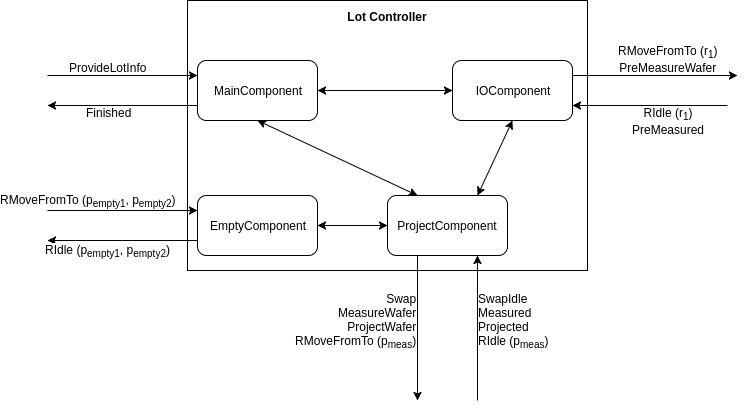
\includegraphics[width=\textwidth]{img/internal_architecture.png}
    \caption{Internal architecture}
    \label{fig:internal_arch}
\end{figure}
Figure~\ref{fig:internal_arch} shows the different internal components as well as the interactions they perform with external systems. 

\subsection{Internal Interactions}
The four internal components will run as parallel processes.
These processes need a way to communicate with each other.
When communication takes place, one process will send information to another process which receives that information.
These send and receive actions need to take place simultaneously.
Such a multi-action can also be described as a single communication action.
The text below describes the communication actions between two components.
Each first mentioned component will send the information, whereas the second mentioned component will receive the sent information.
In our mCRL2~model (see Appendix~\ref{sec:model}) a send action is prefixed by an `s' and a receive action is prefixed by an `r'.
The allowed actions are all external interactions and communication actions.
All communication actions listed below cannot be observed by the outside world and thus can be hidden using the internal $\tau$-action.

\textbf{MainComponent to IOComponent:}
\begin{itemize}
    \item $\mathit{AvailableWafers}(n)$\\
    Communicates the amount of wafers that are on the current lot where $n \in \mathbb{N}$ is the amount of wafers.
\end{itemize}

\textbf{IOComponent to MainComponent:}
\begin{itemize}
    \item $\mathit{CompletedLot}$\\
    Indicates that all the wafers on the current lot are placed into the tray.
\end{itemize}

\textbf{MainComponent to ProjectComponent:}
\begin{itemize}
    \item $\mathit{ChangeConfig}(r, c)$\\
    Communicate a change in lot configuration which includes the recipe $r \in Q$ as well as the need for calibration $c \in \mathbb{B}$.
\end{itemize}

\textbf{ProjectComponent to MainComponent:}
\begin{itemize}
    \item $\mathit{ChangedConfig}$\\
    Indicates that the configuration has been changed.
\end{itemize}

\textbf{IOComponent to ProjectComponent:}
\begin{itemize}
    \item $\mathit{WaferReadyAtChuckIn}$\\
    Indicates that a wafer is at $p_\mathit{in}$ which has been pre-measured.
    \item $\mathit{WaferTakenAtChuckOut}$\\
    Indicates that the wafer which was on $p_\mathit{out}$ has been placed into the tray.
\end{itemize}

\textbf{ProjectComponent to IOComponent:}
\begin{itemize}
    \item $\mathit{WaferReadyAtChuckOut}$\\
    Indicates that a wafer is at $p_\mathit{out}$ which has been projected.
    \item $\mathit{WaferTakenAtChuckIn}$\\
    Indicates that the wafer which was on $p_\mathit{in}$ has been moved to $p_\mathit{meas}$.
\end{itemize}

\textbf{ProjectComponent to EmptyComponent:}
\begin{itemize}
    \item $\mathit{ProvideClosingWafer}$\\
    Request a closing wafer to be placed at $p_\mathit{meas}$.
    \item $\mathit{StoreClosingWafer}$\\
    Request the closing wafer to be removed from $p_\mathit{meas}$.
\end{itemize}

\textbf{EmptyComponent to ProjectComponent:}
\begin{itemize}
    \item $\mathit{ProvidedClosingWafer}$\\
    Indicates that a closing wafer has been placed at $p_\mathit{meas}$.
    \item $\mathit{StoredClosingWafer}$\\
    Indicates that a closing wafer has been removed from $p_\mathit{meas}$.
\end{itemize}

    \section{Modal Formulas}\label{sec:modal_formulas}
\begin{enumerate}
    \item $[!Finished^{*}]<true^{*} \cdot Finished>true$
    \item \begin{enumerate}
        \item \begin{align*}
            &\nu X(i:Int = 0) . & \\
            &[RMoveFromTo(r_1, p_\mathit{tray}, p_\mathit{in})]X(i+1) \\
            &\wedge [RMoveFromTo(r_1, p_\mathit{out}, Tray)]X(i-1) \\
            &\wedge [\overline{\{Finished,RMoveFromTo(r_1, p_\mathit{tray}, p_\mathit{in}),RMoveFromTo(r_1, p_\mathit{out}, Tray)\}}]X(i) \\
            &\wedge [Finished](i \approx 0)
        \end{align*}
        \item \begin{align*}
            &\nu X(C : Set(P) = \{p_\mathit{meas},p_\mathit{proj}\}).\\
            & \forall r:R, p_1, p_2 : P . [RMoveFromTo(r, p_1, p_2)](if(p_1 \in C, X(C\backslash\{p_1\}\cup\{p_2\}), X(C))\\
            &\wedge ((p_\mathit{meas} \in C \wedge p_\mathit{proj} \in C) \implies [Swap]X(C))\\
            &\wedge ((p_\mathit{meas} \notin C \wedge p_\mathit{proj} \notin C) \implies [Swap]X(C))\\
            &\wedge ((p_\mathit{meas} \notin C \wedge p_\mathit{proj} \in C) \implies [Swap]X(C\backslash\{p_\mathit{proj}\} \cup \{p_\mathit{meas}\}))\\
            &\wedge ((p_\mathit{meas} \in C \wedge p_\mathit{proj} \notin C) \implies [Swap]X(C\backslash\{p_\mathit{meas}\} \cup \{p_\mathit{proj}\}))\\
            &\wedge [\overline{\{RMoveFromTo, Swap, Finished\}}]X(C)\\
            &\wedge [Finished](C \approx \{p_\mathit{meas},p_\mathit{proj}\})
        \end{align*}
        \item Follows from a and b
    \end{enumerate}
    \item \begin{enumerate}
        \item $\forall r:R., p_1,p_2,p_1',p+2':P.[true^{*}\cdot RMoveFromTo(r, p_1, p_2) \cdot \overline{RIdle(r, p_1, p_2)}^{*} \cdot RMoveFromTo(r, p_1', p_2')]false$
        \item $[true^{*}\cdot Swap \cdot \overline{Swapped}^{*} \cdot Swap]false$
        \item $[true^{*}\cdot PreMeasureWafer \cdot \overline{PreMeasured}^{*} \cdot PreMeasureWafer]false$
        \item $[true^{*}\cdot MeasureWafer \cdot \overline{Measured}^{*} \cdot MeasureWafer]false$
        \item $[true^{*}\cdot ProjectWafer \cdot \overline{Projected}^{*} \cdot ProjectWafer]false$
        \item $[true^{*}\cdot Calibrate \cdot \overline{Calibrated}^{*} \cdot Calibrate]false$
    \end{enumerate}
        \item \begin{align*}
            &\nu X(w:T\mapsto \mathbb{B} = (\lambda p:T.false)[p_\mathit{meas} \rightarrow true][p_\mathit{proj} \rightarrow true]). \\
            &\wedge \forall r:R, p_1,p_2 :T.[RMoveFromTo(r, p_1,p_2)]((p_1 \approx p_\textit{tray} \vee w(p_1)) \wedge (p_2 \approx p_\textit{tray} \vee \lnot w(p_2)) \wedge X(w[p_1\rightarrow false]))\\
            &\wedge \forall r:R, p_1,p_2 :T.[RIdle(r, p_1,p_2)]X(w[p_2\rightarrow true])\\
            &\wedge [\overline{RMoveFromTo, RIdle}]X(w)
        \end{align*}
    \item $\forall r,r' :R, p_1,p_1' : T, p_2:P.[true^{*}\cdot RIdle(r, p_1, p_2) \cdot 	(\forall r'':R, p_3:T. \overline{RMoveFromTo(r'', p_2, p_3)})\cdot RIdle(r', p_1', p_2)]false$
    \item $[true^{*}\cdot RMoveFromTo(r_1, p_\mathit{tray}, p_\mathit{in}) \cdot \overline{PreMeasured}^{*} \cdot RMoveFromTo(r_2, p_\mathit{in}, p_\mathit{meas})]false$
    \item \begin{align*}
    	&\nu X(mm:\mathbb{B} = false, pm:\mathbb{B}=false).\\
    	&[Measured]X(true, pm)\\
    	&\wedge [Swapped]X(pm, mm)\\
    	&\wedge \forall r:R, p_1, p_2:T.[RMoveFromTo(r, p_1, p_2)](if(p_1 \approx p_\mathit{meas}, X(false, pm), X(mm, pm))\\
    	&\wedge [\overline{\{Measured, Swapped, RMoveFromTo, Project\}}]X(mm, pm)\\
    	&\wedge [Project](pm \approx true \wedge X(mm, pm))
    \end{align*}
        \item \begin{align*}
            &\nu X(C : Set(P) = \{p_\mathit{meas},p_\mathit{proj}\}).\\
            & \forall r:R, p_1, p_2 : P . [RMoveFromTo(r, p_1, p_2)]&((p_2 \in \{p_\mathit{empty1}, p_\mathit{empty2}\} \implies p_1 \in C)\\
            &&\wedge (if(p_1 \in C, X(C\backslash\{p_1\}\cup\{p_2\}), X(C))) \\
            &\wedge ((p_\mathit{meas} \in C \wedge p_\mathit{proj} \in C) \implies [Swap]X(C))\\
            &\wedge ((p_\mathit{meas} \notin C \wedge p_\mathit{proj} \notin C) \implies [Swap]X(C))\\
            &\wedge ((p_\mathit{meas} \notin C \wedge p_\mathit{proj} \in C) \implies [Swap]X(C\backslash\{p_\mathit{proj}\} \cup \{p_\mathit{meas}\}))\\
            &\wedge ((p_\mathit{meas} \in C \wedge p_\mathit{proj} \notin C) \implies [Swap]X(C\backslash\{p_\mathit{meas}\} \cup \{p_\mathit{proj}\}))\\
            &\wedge [\overline{\{RMoveFromTo, Swap, Finished\}}]X(C)
        \end{align*}
    \item \begin{align*}
	    &[true^{*}\cdot MeasureWafer\cdot \overline{Measured}^{*}\cdot Swap]false\\
		&\wedge [true^{*}\cdot ProjectWafer\cdot \overline{Projected}^{*}\cdot Swap]false\\
	    &\wedge [true^{*}\cdot Calibrate\cdot \overline{Calibrated}^{*}\cdot Swap]false
    \end{align*}
    \item Implemented by 4.
    \item \begin{align*}
            &\nu X(w:T\mapsto \mathbb{B} = (\lambda p:T.false)[p_\mathit{meas} \rightarrow true][p_\mathit{proj} \rightarrow true]). \\
            &\wedge \forall r:R, p_1,p_2 :T.[RMoveFromTo(r, p_1,p_2)]X(w[p_1\rightarrow false])\\
            &\wedge \forall r:R, p_1,p_2 :T.[RIdle(r, p_1,p_2)]X(w[p_2\rightarrow true])\\
            &\wedge [\overline{RMoveFromTo, RIdle}]X(w)\\
            &\wedge [Swap](w(p_\textit{meas}) \wedge w(p_\textit{proj}))
        \end{align*}
    \item \begin{align*}
    	&\nu X(rec:Q = Recipe_3, even:\mathbb{B} = true).\\
  		&\forall n:\mathbb{N}, r:Q, b:\mathbb{B}.[ProvideLotInfo(n,r,b)](X(r,even))\\
  		&\wedge [Swapped]X(rec, \lnot even)\\
  		&\wedge [\overline{\{ProvideLotInfo, Swapped, Project\}}]X(rec, even)\\
  		&\wedge [Project]((rec \approx Recipe_1 \implies even) \wedge (rec \approx Recipe_2 \implies \lnot even) \wedge X(rec, even))
    \end{align*}
    \item \begin{align*}
            &\nu X(w:T\mapsto \mathbb{B} = (\lambda p:T.false)[p_\mathit{meas} \rightarrow true][p_\mathit{proj} \rightarrow true]). \\
            &\wedge \forall r:R, p_1,p_2 :T.[RMoveFromTo(r, p_1,p_2)]X(w[p_1\rightarrow false])\\
            &\wedge \forall r:R, p_1,p_2 :T.[RIdle(r, p_1,p_2)]X(w[p_2\rightarrow true])\\
            &\wedge [\overline{RMoveFromTo, RIdle}]X(w)\\
            &\wedge [MeasureWafer](w(p_\textit{meas}))\\
            \wedge\\
            &\nu X(C : Set(P) = \{p_\mathit{meas},p_\mathit{proj}\}).\\
            & \forall r:R, p_1, p_2 : P . [RMoveFromTo(r, p_1, p_2)](if(p_1 \in C, X(C\backslash\{p_1\}\cup\{p_2\}), X(C))\\
            &\wedge ((p_\mathit{meas} \in C \wedge p_\mathit{proj} \in C) \implies [Swap]X(C))\\
            &\wedge ((p_\mathit{meas} \notin C \wedge p_\mathit{proj} \notin C) \implies [Swap]X(C))\\
            &\wedge ((p_\mathit{meas} \notin C \wedge p_\mathit{proj} \in C) \implies [Swap]X(C\backslash\{p_\mathit{proj}\} \cup \{p_\mathit{meas}\}))\\
            &\wedge ((p_\mathit{meas} \in C \wedge p_\mathit{proj} \notin C) \implies [Swap]X(C\backslash\{p_\mathit{meas}\} \cup \{p_\mathit{proj}\}))\\
            &\wedge [\overline{\{RMoveFromTo, Swap\}}]X(C)\\
            &\wedge [MeasureWafer](p_\mathit{meas} \notin C)
        \end{align*}
    \item \begin{align*}
    		&\nu X(C : Set(P) = \{p_\mathit{meas},p_\mathit{proj}\}).\\
            & \forall r:R, p_1, p_2 : P . [RMoveFromTo(r, p_1, p_2)](if(p_1 \in C, X(C\backslash\{p_1\}\cup\{p_2\}), X(C))\\
            &\wedge ((p_\mathit{meas} \in C \wedge p_\mathit{proj} \in C) \implies [Swap]X(C))\\
            &\wedge ((p_\mathit{meas} \notin C \wedge p_\mathit{proj} \notin C) \implies [Swap]X(C))\\
            &\wedge ((p_\mathit{meas} \notin C \wedge p_\mathit{proj} \in C) \implies [Swap]X(C\backslash\{p_\mathit{proj}\} \cup \{p_\mathit{meas}\}))\\
            &\wedge ((p_\mathit{meas} \in C \wedge p_\mathit{proj} \notin C) \implies [Swap]X(C\backslash\{p_\mathit{meas}\} \cup \{p_\mathit{proj}\}))\\
            &\wedge [\overline{\{RMoveFromTo, Swap\}}]X(C)\\
            &\wedge [ProjectWafer](p_\mathit{proj})
        \end{align*}
    \item \begin{align*}
    		&\nu X(C : Set(P) = \{p_\mathit{meas},p_\mathit{proj}\}).\\
            & \forall r:R, p_1, p_2 : P . [RMoveFromTo(r, p_1, p_2)](if(p_1 \in C, X(C\backslash\{p_1\}\cup\{p_2\}), X(C))\\
            &\wedge ((p_\mathit{meas} \in C \wedge p_\mathit{proj} \in C) \implies [Swap]X(C))\\
            &\wedge ((p_\mathit{meas} \notin C \wedge p_\mathit{proj} \notin C) \implies [Swap]X(C))\\
            &\wedge ((p_\mathit{meas} \notin C \wedge p_\mathit{proj} \in C) \implies [Swap]X(C\backslash\{p_\mathit{proj}\} \cup \{p_\mathit{meas}\}))\\
            &\wedge ((p_\mathit{meas} \in C \wedge p_\mathit{proj} \notin C) \implies [Swap]X(C\backslash\{p_\mathit{meas}\} \cup \{p_\mathit{proj}\}))\\
            &\wedge [\overline{\{RMoveFromTo, Swap\}}]X(C)\\
            &\wedge [RMoveFrom(r_3,p_\mathit{meas}, p_\mathit{out})](p_\mathit{meas} \notin C)
        \end{align*}
    \item $\forall n:\mathbb{N},q:Q.[true^{*}\cdot ProvideLotInfo(n,q,true)\cdot \overline{Calibrated}\cdot RMoveFromTo(r_2, p_\mathit{in}, p_\mathit{meas})]false$
    \item \begin{align*}
    		&\nu X(C : Set(P) = \{p_\mathit{meas},p_\mathit{proj}\}).\\
            & \forall r:R, p_1, p_2 : P . [RMoveFromTo(r, p_1, p_2)](if(p_1 \in C, X(C\backslash\{p_1\}\cup\{p_2\}), X(C))\\
            &\wedge ((p_\mathit{meas} \in C \wedge p_\mathit{proj} \in C) \implies [Swap]X(C))\\
            &\wedge ((p_\mathit{meas} \notin C \wedge p_\mathit{proj} \notin C) \implies [Swap]X(C))\\
            &\wedge ((p_\mathit{meas} \notin C \wedge p_\mathit{proj} \in C) \implies [Swap]X(C\backslash\{p_\mathit{proj}\} \cup \{p_\mathit{meas}\}))\\
            &\wedge ((p_\mathit{meas} \in C \wedge p_\mathit{proj} \notin C) \implies [Swap]X(C\backslash\{p_\mathit{meas}\} \cup \{p_\mathit{proj}\}))\\
            &\wedge [\overline{\{RMoveFromTo, Swap\}}]X(C)\\
            &\wedge [Calibrate](p_\mathit{meas} \in C \wedge p_\mathit{proj} \in C)
        \end{align*}
    \item \begin{align*}
    	&\nu X(mp:\mathbb{B} = false, pp:\mathbb{B}=false).\\
    	&[Projected]X(mp, true)\\
    	&\wedge [Swapped]X(pp, mp)\\
    	&\wedge [RMoveFromTo(r_2, p_\mathit{meas}, p_\mathit{out})](mp \wedge X(false, pp))\\
    	&\wedge [\overline{\{Projected, Swapped, RMoveFromTo(r_2, p_\mathit{meas}, p_\mathit{out})\}}]X(mp, pp)
    \end{align*}
\end{enumerate}
    \section{Verification}\label{sec:results}
The lot controller requires information about the lots on the tray through \textit{ProvideLotInfo} to run. \textit{ProvideLotInfo} takes 3 arguments: a natural number, a recipe and a boolean. Furthermore \textit{ProvideLotInfo} represents a single lot, the only restriction to the number of lots is that it is finite. The model can't be checked for all possibile inputs therefor the process \textit{TrayInputLoop} is declared which provides the lot controller with \text{ProvideLotInfo} commands. \textit{TrayInputLoop} takes 2 parameters: $\mathit{maxLots} \in \mathbb{N}$ and $\mathit{maxWafersPerLot} \in \mathbb{N}$. \textit{TrayInputLoop} calls \textit{ProvideLotInfo} with at most $\mathit{maxWafersPerLot}$ wafers at most $\mathit{maxLots}$ times. The number of possible traces for \textit{TrayInputLoop} is:
$$(\mathit{maxLots}+1) \cdot 3 \cdot \mathit{maxWafersPerLot} \cdot 2$$
This formula represent the possible number of lots multiplied by the number of recipes multiplied by the maximum number of wafers per lot multiplied by two (i.e. whether to calibrate or not)). $\mathit{maxLots} = 10$ and $\mathit{maxWafersPerLot} = 24$ are used during validation of the model.

\subsection{Execution}
The model is verified on a machine with the following specifications:\\
Operating system: Ubuntu 17.04\\
Cpu: Intel(R) Pentium(R) CPU B980 @ 2.40GHz\\
RAM: 8 GB\\

The mCRL2 toolset version "201707.1 (Release)" was used to verify the models.

The following command is used to generate the \textit{lps} file:\\
\begin{lstlisting}[frame=single,caption={mcf2lps}]
mcrl22lps -lregular2 "${MCRL2_NAME}.mcrl2" "${MCRL2_NAME}.lps"
\end{lstlisting}
Where \$\{MCRL2\_NAME\}.mcrl2 refers to the mcrl2 file (without filetype suffix) containing the model which can be found in appendix \ref{sec:model}.\\
The following command is used to verify a \textit{mcf} file:\\
\begin{lstlisting}[frame=single,caption={mcf check}] 
lps2pbes "${MCRL2_NAME}.lps" "${file%.mcf}.pbes" "-f${file}" \
                && pbes2bool "${file%.mcf}.pbes" --rewriter=jittyc
\end{lstlisting}
Where \$\{file\} refers to the mcf file containing the a modal formula which can be found in appendix \ref{sec:mcf}.\\
\subsection{Results}
First the \text{lps} file was generated using the \text{mcf2lps} command above. Second every \textit{mcf} file is checked using the \textit{mcf check} command. The following table describes the results.
\begin{table}[h]
\label{my-label}
\begin{tabular}{|l|l|l|}
\hline
\textbf{Mcf} & \textbf{Result} & \textbf{Execution time} \\ \hline
Auxilary 1 & true & 4m44s \\ \hline
Requirement 1 & true & 0m43s \\ \hline
Requirement 2a & true & 0m41s \\ \hline
Requirement 2b & true & 1m49s \\ \hline
Requirement 2c & true & 0m12s \\ \hline
Requirement 3a & true & 2m48s \\ \hline
Requirement 3b & true & 0m37s \\ \hline
Requirement 3c & true & 0m38s \\ \hline
Requirement 3d & true & 0m34s \\ \hline
Requirement 3e & true & 0m33s \\ \hline
Requirement 3f & true & 0m33s \\ \hline
Requirement 4 & true & 6m27s \\ \hline
Requirement 5 & true & 7m22s \\ \hline
Requirement 6 & true & 0m42s \\ \hline
Requirement 7 & true & 1m44s \\ \hline
Requirement 8 & true & 1m57s \\ \hline
Requirement 9 & true & 1m03s \\ \hline
Requirement 10 & true & 0m48s \\ \hline
Requirement 11 & true & 5m47s \\ \hline
Requirement 12 & true & 0m31s \\ \hline
Requirement 13 & true & 8m44s \\ \hline
Requirement 14 & true & 1m53s \\ \hline
Requirement 15 & true & 1m57s \\ \hline
Requirement 16 & true & 0m37s \\ \hline
Requirement 17 & true & 1m58s \\ \hline
Requirement 18 & true & 2m17s \\ \hline
\end{tabular}
\end{table}

    \newpage
    \appendix
    \section{Model}\label{sec:model}
    \lstinputlisting{../src/model.mcrl2}

    \section{Verification}\label{sec:mcf}
    \subsection{Requirement 1}
    \lstinputlisting{../src/requirements/req1.mcf}

    \subsection{Requirement 2}
    \subsubsection{Requirement 2a}
    \lstinputlisting{../src/requirements/req2a.mcf}

    \subsubsection{Requirement 2b}
    \lstinputlisting{../src/requirements/req2b.mcf}

    \subsubsection{Requirement 2c}

    \subsection{Requirement 3}
    \subsubsection{Requirement 3a}
    \lstinputlisting{../src/requirements/req3a.mcf}

    \subsubsection{Requirement 3b}
    \lstinputlisting{../src/requirements/req3b.mcf}

    \subsubsection{Requirement 3c}
    \lstinputlisting{../src/requirements/req3c.mcf}

    \subsubsection{Requirement 3d}
    \lstinputlisting{../src/requirements/req3d.mcf}

    \subsubsection{Requirement 3e}
    \lstinputlisting{../src/requirements/req3e.mcf}

    \subsubsection{Requirement 3f}
    \lstinputlisting{../src/requirements/req3f.mcf}

    \subsection{Requirement 4}
    \lstinputlisting{../src/requirements/req4.mcf}

    \subsection{Requirement 5}
    \lstinputlisting{../src/requirements/req5.mcf}

    \subsection{Requirement 6}
    \lstinputlisting{../src/requirements/req6.mcf}

    \subsection{Requirement 7}
    \lstinputlisting{../src/requirements/req7.mcf}

    \subsection{Requirement 8}
    \lstinputlisting{../src/requirements/req8.mcf}

    \subsection{Requirement 9}
    \lstinputlisting{../src/requirements/req9.mcf}

    \subsection{Requirement 10}
    \lstinputlisting{../src/requirements/req10.mcf}

    \subsection{Requirement 11}
    \lstinputlisting{../src/requirements/req11.mcf}

    \subsection{Requirement 12}
    \lstinputlisting{../src/requirements/req12.mcf}

    \subsection{Requirement 13}
    \lstinputlisting{../src/requirements/req13.mcf}

    \subsection{Requirement 14}
    \lstinputlisting{../src/requirements/req14.mcf}

    \subsection{Requirement 15}
    \lstinputlisting{../src/requirements/req15.mcf}

    \subsection{Requirement 16}
    \lstinputlisting{../src/requirements/req16.mcf}

    \subsection{Requirement 17}
    \lstinputlisting{../src/requirements/req17.mcf}

    \subsection{Requirement 18}
    \lstinputlisting{../src/requirements/req18.mcf}
    
    \subsection{Auxilary 1}
    \lstinputlisting{../src/requirements/reqaux1.mcf}

\end{document}
